% Chapter 1

\chapter{Analysis} % Chapter title

\label{ch:architecture} % For referencing the chapter elsewhere, use \autoref{ch:architecture} 

%----------------------------------------------------------------------------------------

\section{Installation structure}

Now that the application has been implemented, it is relevant to analyze how the entire installation structure. \\

A variety of softare packages have been installed on the server, these being PyWPS, Flask, Apache2 and GRASS.
Debugging: When the server has been installed, it runs on it's own, and not much else has to be manipulated with from then on. When the process fail for some reason, it can be relevant to troubleshoot the problem by reading the error log. Both Apache and PyWPS have error logs that can provide information about the situation, which can help to fix the error. The logs for both of these critical components can be found in the following directories:\\


\dirtree{%
.1 /.
.2 /var/.
.3 /www/.
.4 /html.
.5 /pywps/.
.6 pywps\.log.
.3 /log/.
.4 /apache2/.
.5 error\.log.
}\\
\\

Accessing the PyWPS installation: When wanting to change, or modify, some of the functionality of PyWPS, it is necessary to access the server and perform the changes here. The setup is displayed in Figure XXX. 


\dirtree{%
.1 /.
.2 /var/.
.3 /www/.
.4 /html.
.5 /pywps/.
.6 pywps\.log.
.6 pywps.cfg.
.6 /processes/.
.7 \_\_init\_\_.py.
.7 process1\.py.
}\\
\\

When adding or removing processes, it has to be done in the processes folder. The process is added (or removed) from the drive, and the \_\_init\_\_.py file is modified to reflect the change that has occurred in the drive.

A variety of serverside settings can be managed from the pywps.cfg file, for instance the maximum allowed filesize of a DEM used as input, or the location of PyWPS outputs.

Flask is installed in the directories shown on Figure XXX.\\



\dirtree{%
.1 /.
.2 /var/.
.3 /www/.
.4 /html.
.5 /FlaskApp/.
.5 flaskapp\.wsgi.
.6 /FlaskApp/.
.7 /templates/.
.7 /images/.
.7 /static/.
.7 \_\_init\_\_.py.
}\\
\\


It is within the \_\_init\_\_.py file that most changes mentioned in the Implementation section have been performed. The templates folder contains the templates used to display HTML. The static folder contains a variety of static content, such as the jQuery and CSS libraries. A functionality of Flask is that content on the server that isn't directly served by the user, isn't meant to be accessible. But if it is placed within the static folder, and the url to the content is known, it can be accessed from “outside”. The outputs of the PyWPS service are therefore directed to a subdirectory of the static folder, so that we can easily access the data through the website front-end.
The images folder is used to store the DEM the user uploads, and works with through the entire process.\\

\dirtree{%
.1 /.
.2 /home/.
.3 /ubuntu/.
.4 \.grassrc6.
.4 /grassdata/.
.5 <LOCATION>.
.6 <MAPSET>.
}\\
\\

The GRASS installation is fairly simple, and after the initial setup is not touched, even when adding new functionalities. The grassdata folder normally contains the various locations and mapsets that are used by the user. In our case the folder only contains one LOCATION, projected to WGS84. This will be used by the PyWPS process to work with the data in question. 
The .grassrc6 folder contains some settings that are needed for GRASS to function properly.

\section{Architecture}
\begin{figure}[h!]
\centering
	{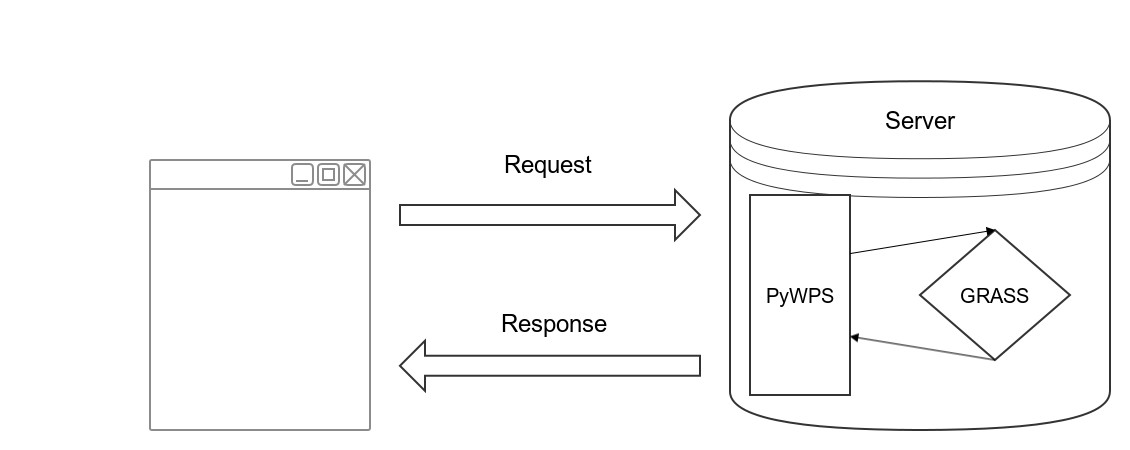
\includegraphics[width=\linewidth]{gfx/Analysis_Architecture/grass_pywps.png}}
\caption{The architecture of the software}
\label{fig:grass_archi}
\end{figure}


\section{User experience}
In this part of the report we will present  how our web service works for the point of view of the user. What we will do, is try to demonstrate as detailed as possible the actual results of the phases we described on the previous chapter. We will also include a step-by-step guideline on how the service should be used and what actions are necessary for the user to follow in order to get the best results possible out of this process. But before we go in depth of the structure of the website, we will take a look at the overview of the setup, as seen on \autoref{analysis_1}

\begin{figure}[h!]
\centering
	{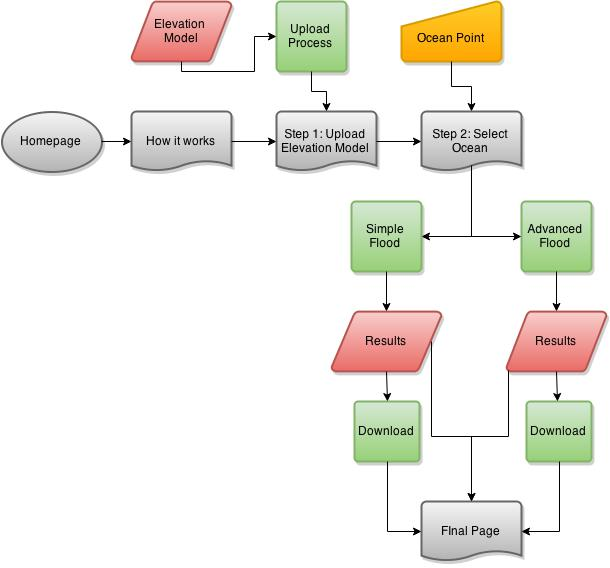
\includegraphics[width=0.75\linewidth]{gfx/Analysis_Website/1.jpg}}
\caption{Overall workflow of the application}
\label{fig:analysis_1}
\end{figure}

We begin by presenting the first page the user will see when they visit our website. The url that leads to the homepage of the application is http://52.17.144.192/. The first page is then displayed that provides information about the website such as its name and a basic description of what services it offers (\autoref{fig:analysis_2}

\begin{figure}[h!]
\centering
	{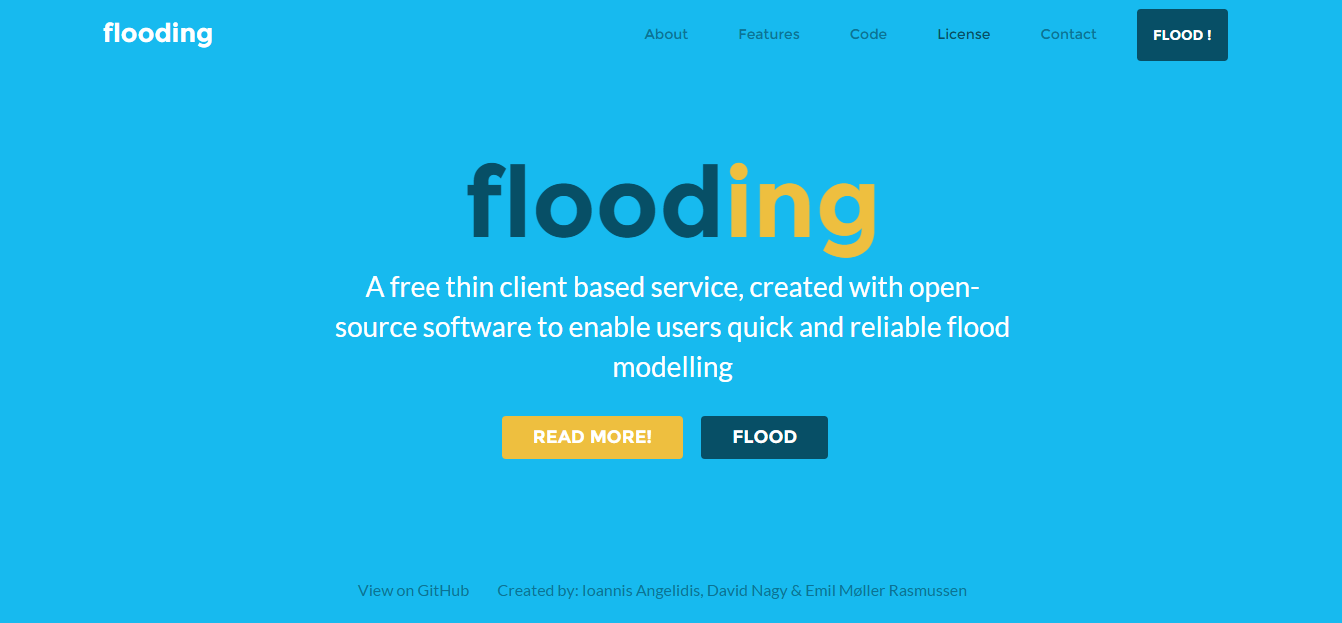
\includegraphics[width=0.75\linewidth]{gfx/Analysis_Website/2.png}}
\caption{Homepage of the application}
\label{fig:analysis_2}
\end{figure}

Lower on the same page, we provide the user with detailed information about the application. The reason we have created it, who can use it and its most important advantages and features \autoref{fig:analysis_3}


\begin{figure}[h!]
\centering
	{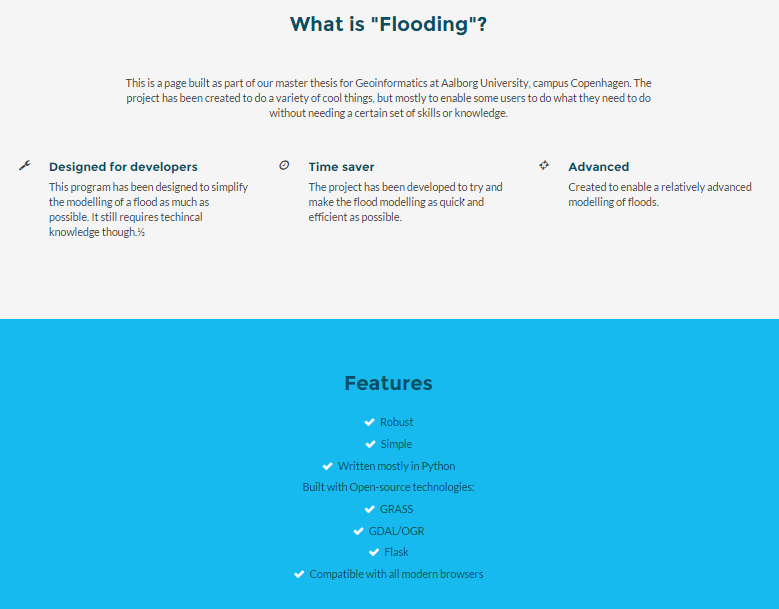
\includegraphics[width=0.75\linewidth]{gfx/Analysis_Website/3.png}}
\caption{Details and characteristics of the application}
\label{fig:analysis_3}
\end{figure}\\

On the final part of the page, we provide the user with small examples of the programming languages, frameworks and other tools we used on order to create this service 
\autoref{fig:analysis_4}

\begin{figure}[h!]
\centering
	{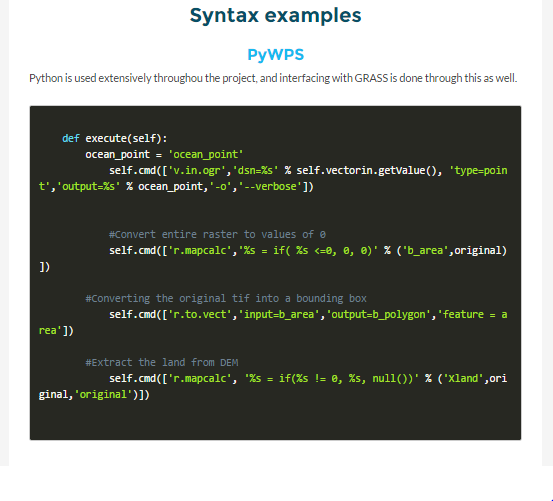
\includegraphics[width=0.75\linewidth]{gfx/Analysis_Website/4.png}}
\caption{Examples of scripts in use}
\label{fig:analysis_4}
\end{figure}

In order to proceed with the actual simulation the option FLOOD on the first part of the page has to be chosen. That will create a new tab on the browser that leads to the second part of the website (\autoref{analysis_5}). This part is a guided process of the flood simulation that follows. By clicking on the Commence flooding option, the initial part of the flood commences.

\begin{figure}[h!]
\centering
	{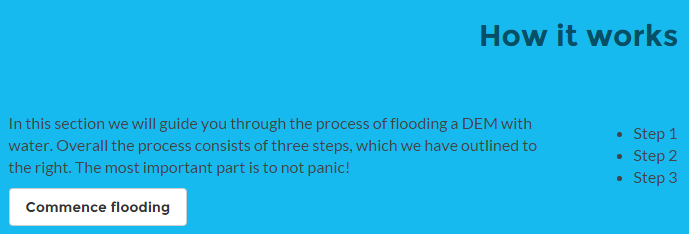
\includegraphics[width=0.75\linewidth]{gfx/Analysis_Website/5.png}}
\caption{Introduction to flooding simulation}
\label{fig:analysis_5}
\end{figure}

The process starts with requesting the user for the necessary input in order for the application to run (\autoref{fig_analysis_6}). As mentioned in previous parts of the report, that necessary input is an elevation model. 

\begin{figure}[h!]
\centering
	{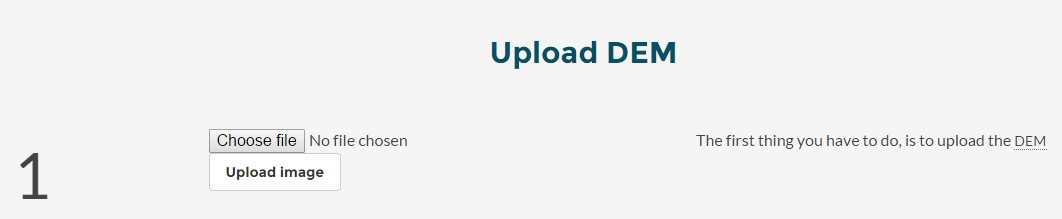
\includegraphics[width=0.75\linewidth]{gfx/Analysis_Website/6.png}}
\caption{Step 1 upload Digital Elevation Model}
\label{fig:analysis_6}
\end{figure}

Once the user chooses an elevation model from his local hard drive and then uploads it, the second step is initialized (\autoref{fig:analysis_7}). 


\begin{figure}[h!]
\centering
	{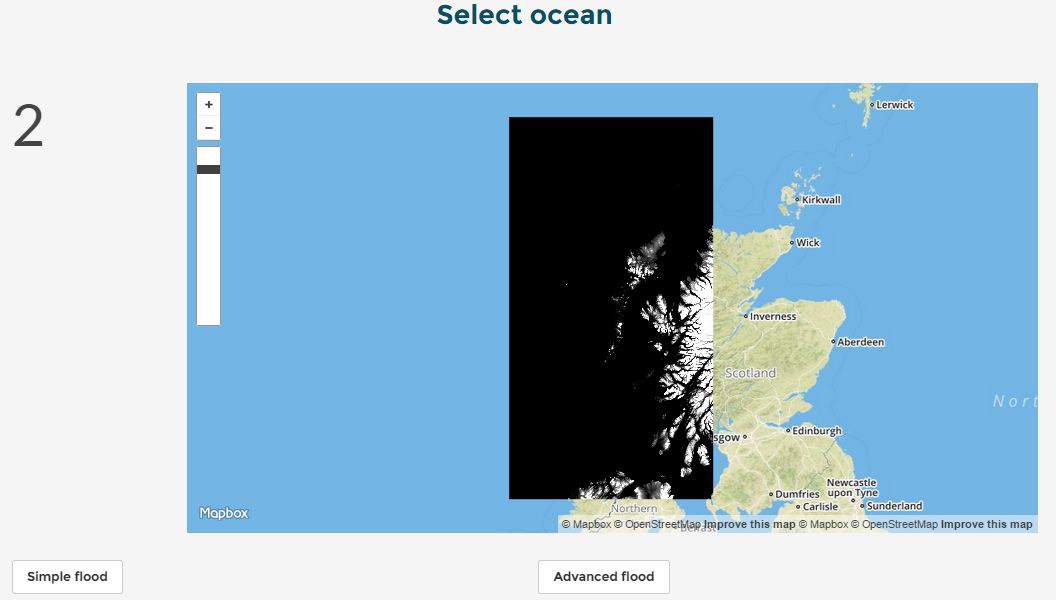
\includegraphics[width=0.75\linewidth]{gfx/Analysis_Website/7.png}}
\caption{Step 2 display uploaded elevation model and insert point to designate origin of flood}
\label{fig:analysis_7}
\end{figure}

the application the user is called to provide it with the ocean. In other words, where he wants the flood to originate from. By simply clicking on the map, that point is created. 
Finally, the user then has to decide which type of process he/she wishes to perform. The simple flood option will instantly fill the elevation model with a predefined level of water and display the results on a map on the third step (\autoref{fig:analysis_8}).

\begin{figure}[h!]
\centering
	{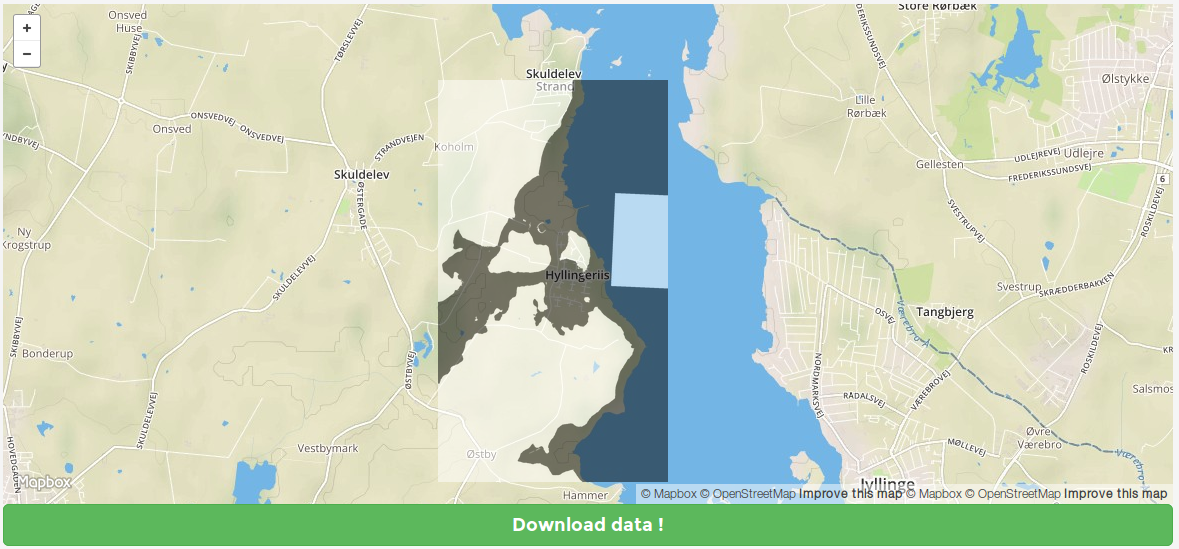
\includegraphics[width=0.75\linewidth]{gfx/Analysis_Website/8.png}}
\caption{Results of the simple flood option}
\label{fig:analysis_8}
\end{figure}
